\documentclass[12pt] {article}
\usepackage[margin=1in]{geometry} %one inch margins
\renewcommand{\baselinestretch}{1.5} %double space, safe for fancy headers
\usepackage{pslatex} %Times font
\usepackage{graphicx} %for figures
\usepackage{enumerate} %for lists
\usepackage{fancyhdr} %header
\pagestyle{fancy}
\usepackage[font={small,sf},format=plain,labelfont=bf,up]{caption}
\fancyhf{}
\fancyhead[l,lo]{150001C \textit{ Internship Report}} %left top header
\fancyhead[r,ro]{\thepage} %right top header
\usepackage{kernelstyle}
\usepackage{listings}
\usepackage{amsmath,amssymb,amsfonts,amsthm}
\usepackage{graphicx}
% \usepackage[utf8]{inputenc}
\usepackage{float}
\usepackage[caption=false,font=timesnewroman]{subfig}
\usepackage[final]{pdfpages}

\graphicspath{{figures/}}

\usepackage{xcolor}
\usepackage{soul}
\usepackage{hyperref}
\hypersetup{
    colorlinks=true,
    linkcolor=blue,
    filecolor=magenta,      
    urlcolor=cyan,
}
\captionsetup[figure]{labelfont={bf},name={Fig.},labelsep=period}
\captionsetup[table]{labelfont={bf},name={Table.},labelsep=period}
\usepackage{caption}
\usepackage{chngcntr} 
\counterwithin{figure}{section}
\counterwithin{table}{section}


\usepackage{algorithmic}
\usepackage[ruled, noend,lined,linesnumbered]{algorithm2e}

\newcommand{\hlc}[2][yellow]{{%
    \colorlet{foo}{#1}%
    \sethlcolor{foo}\hl{#2}}%
}

\usepackage{hyperref}
\hypersetup{
   colorlinks=true,
   linkcolor = black,
   citecolor=Green
}


\title{INTERNSHIP REPORT}


\definecolor{hgray}{RGB}{130,130,130}
\definecolor{hred}{RGB}{136,0,0}
\definecolor{black}{RGB}{0,0,0}
\definecolor{Green}{RGB}{0,255,0}

\usepackage[T1]{fontenc}
\usepackage[tableposition=top]{caption}
\usepackage{rotating}
\usepackage{color, colortbl}
\usepackage{booktabs, array, dcolumn}
\usepackage{tikz}
\usepackage{graphicx}
\usepackage{pgf-umlsd}
\usepackage{multirow}
\usepackage{epsfig}
\usepackage{subfig}
\usepackage{pgfplotstable}
\usepackage{amsfonts}
\usepackage{relsize}
\usepackage{varwidth}
\usepackage{url}
\usepackage{amsmath}
\usepackage{amssymb}
\usepackage{booktabs}
% \usepackage{soul}
\usepackage[normalem]{ulem}
\usepackage{subfig}
\usepackage{kernelstyle}
\definecolor{Gray}{gray}{0.9}
\usepackage{hyperref}
% \usepackage{tabularx}
\usepackage{footnote}

\definecolor{gray1}{gray}{0.9}
\definecolor{gray2}{gray}{0.6}
\definecolor{Gray}{gray}{0.9}


\definecolor{light-gray1}{gray}{0.65}
\definecolor{light-gray2}{gray}{0.95}

%%------------------------ PREAMBLE ENDS ---------------------------

\begin{document}
\pagenumbering{roman} % Start roman numbering


\newpage

\tableofcontents
\newpage
\listoffigures
\listoftables
\newpage
\pagenumbering{arabic}
%!TEX root = ./intern_report.tex
\section*{Preface}

\paragraph{}
Described in this report is the 24 week training experience I had in wave computing/Paraqum Technologies dating from 25.06.2018 to 07.12.2018 for the fulfillment of industrial training requirements of my B.Sc. in Electronics and Telecommunication Engineering. The report consists of 3 main sections as follows

\subsubsection*{Chapter 1: Introduction to Wave computing and Paraqum Technologies}
\paragraph{}
Wave computing is a USA based AI startup and Paraqum Technologies is a Sri Lankan Electronic design startup. Wave is now ranked among the top 25 AI providers of the world~\cite{top25ai} and Paraqum Technologies is highly respected in Sri Lanka as a pioneer of the industry and recieves design contracts from all over the world. Our training was done through a design contract offered to Paraqum by Wave computing.

\subsubsection*{Chapter 2: Training Experience}
\paragraph{}
Even though I was an intern, I was given full exposure to the company workflow. I recieved a full scale project to lead and a support team from all over the world to work with. Everyone in the company were very supportive and friendly. The environment was comfortable to work and the workload was perfectly balanced, demanding yet not overwhelming.

\subsubsection*{Chapter 3: Conclusion}
\paragraph{}
I can say without a doubt, this is one of the best training experiences one can get. The University of Moratuwa Industrial training division, the Department of Electronic and Telecommunication Engineering and National Apprentice and Industrial Training Authority (NAITA) together did their best to provide us with an exceptional experience that will be very useful for the future of our careers.

\newpage
\section*{Acknowledgment}

\paragraph{}
I take this chance to show my gratitude towards everyone that helped make this training possible and facilitated my time with it. First of all I should thank the industrial training division of University of Moratuwa and the National Apprentice and Industrial Training Authority (NAITA) for allowing us to get an industrial training of this magnitude and quality during the time of our studies and always looking out for the wellbeing of the trainees.

\paragraph{}
I also would like to thank the administration and staff of Paraqum Technologies, starting with the CEO Dr. Ajith Pasqual, Manager Eng. Hasanka Sandujith, Eng. Kasun Tharaka who coordinated the internships and all other staff members who helped in a great many ways to make the training a staggering success. 

\paragraph{}
Last but definitely not least, The staff of the Wave computing team (later separated as Wave computing Sri Lanka) were always dedicated to make the training worthwhile for us. I sincerely thank the Senior Director of Software Engineering division of wave computing Eng. Henrik Esbenson, who visited and supervised us from time to time, General manager of Wave computing Eng. Nuwan Gajaweera, Technical leaders Eng. Upul Ekanayaka and Eng. Binu Amarathunga, My supervisors Eng. Achintha Ihalage, Eng. Omega Gamage and SDK team lead Eng. Dakila Serasinghe and all other staff members of wave computing for everything they did for us.

\vspace*{3cm}

\noindent Chinthana Wimalasuriya,\newline
Undergraduate,\newline
Department of Electronics and Telecommunication Engineering,\newline
University of Moratuwa.

\newpage
\section{Introduction to Training Establishment}
%!TEX root = ./intern_report.tex

\subsection{Company Overview}
\subsection{Company History}
\subsection{Organization Structure and Hierarchy}
\subsection{Areas of Interest}
\subsection{Current Situation}
\subsection{Impacts on Sri Lankan Industry}

\subsection{SWOT Analysis}
\subsubsection{Strengths}
\subsubsection{Weaknesses}
\subsubsection{Opportunities}
\subsubsection{Threats}

\subsection{Usefulness to the Country}
\subsection{Suggestions to Improve the Company}

\newpage
\section{Training Experience}
%!TEX root = ./intern_report.tex

\subsection{How I got the Opportunity}

\paragraph{}
After graduation, I wanted to continue doing higher studies and become an academic, rather than settling for a job at a company. Therefore, for my internship, I applied for research opportunities in universities and institutes around the world. I got positive response from two or three institutes, one of them being CSIRO. I sent my CV to Dr. Navinda Kottege from RAG, DATA61, CSIRO in February 2018, requesting a research internship opportunity. He asked me to complete a set of 3 timed tasks online to assess my skills in programming and algorithms. He then interviewed and offered me the position as research intern student in CSIRO for 6 months.

\paragraph{}
Initially I was informed that I am being assigned to the project titled "Computer vision based off-board autonomous UAV Navigation" under the supervision of Mr. Frederick Pauling, a highly capable and friendly senior engineer in DATA61. I was informed that knowledge in ROS (Robot Operating System) and Tensorflow would be necessary, so I spent few weeks learning the basics before the internship.

\paragraph{}
However, when I arrived at CSIRO, Mr. Frederick Pauling had been promoted into the Group Leader of RAG (Robotics and Autonomous systems Group), to lead the cutting edge robotics research in Australia. Therefore, I could not be assigned into the said project under his supervision. As a result, Uvindu and I was assigned under the supervision of Mr. Nicolas Hudson.

\paragraph{}
Mr. Nicolas Hudson arrived CSIRO only few weeks before us, after working as a senior roboticist in NASA's Jet Propulsion Laboratory, Boston Dynamics and Google's Machine Learning Division. In CSIRO he wanted to streamline the workflow of the RAG group and incorporate Machine Learning tools into their workflow seamlessly. He asked us to work with him in one of his experimental projects: "Learning Transfer Across RGB, Thermal and IR Modalities in CNNs". After about a week, Uvindu requested for a project that is more focused on hardware. Hence, he asked us to modify Trailnet for autonomous indoor navigation.

\newpage
\subsection{Trailnet: A Classification Network for Autonomous Trail Navigation}

\subsubsection{Trailnet: An Introduction}

In 2017, four researchers published a paper titled "Toward Low-Flying Autonomous MAV Trail Navigation using Deep Neural Networks for Environmental Awareness"~\cite{trailNet} (Trailnet paper in short) with the funding of NVIDIA. The paper describes the following:

\begin{itemize}
    \item Merits of approaching autonomous navigation as a classification problem
    \item Architecture of their Trailnet CNN, a modified version of Resnet-18. ~\cite{resnet}
    \item Data collection techniques for the Trailnet CNN
    \item Training Trailnet with a relatively small dataset
    \item Hardware hierarchy and the command flow between cameras, NVIDIA Jetson TX2 ~\cite{jetson_tx2} running ROS and the flight control board.
    \item Usage of YOLO for obstacle detection and algorithm for obstacle avoidance.
    \item Results and observations after flying the quadcopter autonomously in the forest trail for several kilometers.
\end{itemize}


\newpage
\subsection{Building Wallie: A Hardware Platform for Data Collection and Deployment}

\begin{figure}[H]
    \centering
    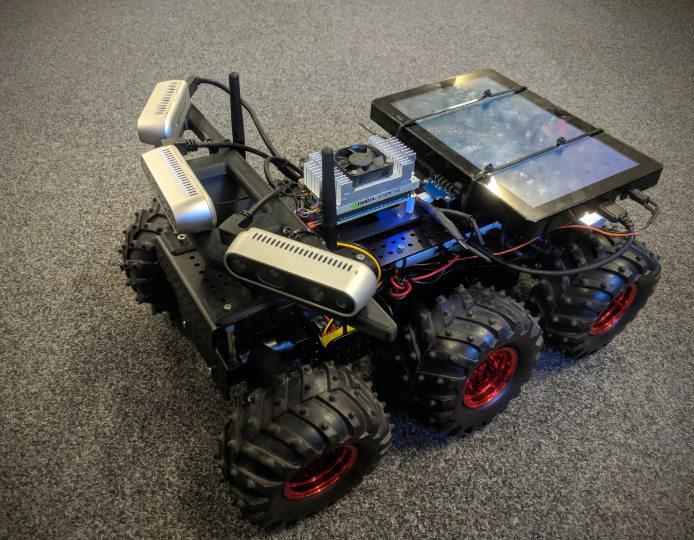
\includegraphics
        [width=10cm]
        {figures/wallie.PNG}
    \caption{Wallie: The Robot \label{Fig:wallie}}\vspace{-4mm}
\end{figure}

\begin{figure}[H]
    \centering
    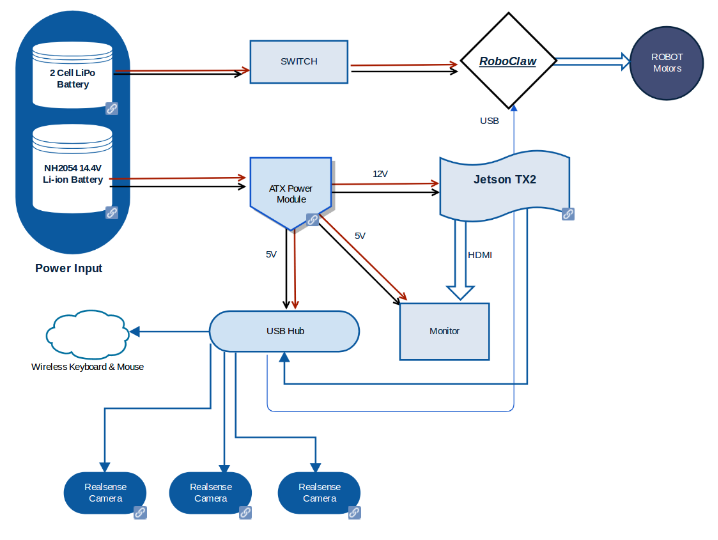
\includegraphics
        [width=10cm]
        {figures/wallie_hardware.PNG}
    \caption{Wallie: Hardware Hierarchy }\vspace{-4mm}
\end{figure}


\subsubsection*{NVIDIA Jetson TX2}

\begin{figure}[H]
    \centering
    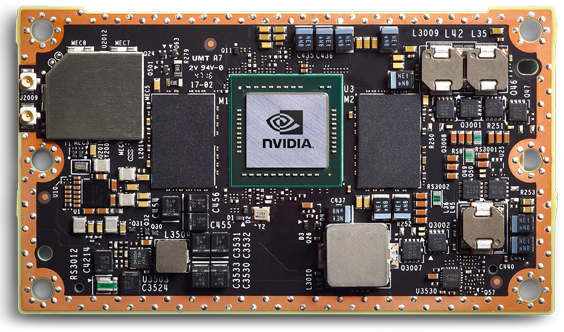
\includegraphics
        [width=8cm]
        {figures/jetson.png}
    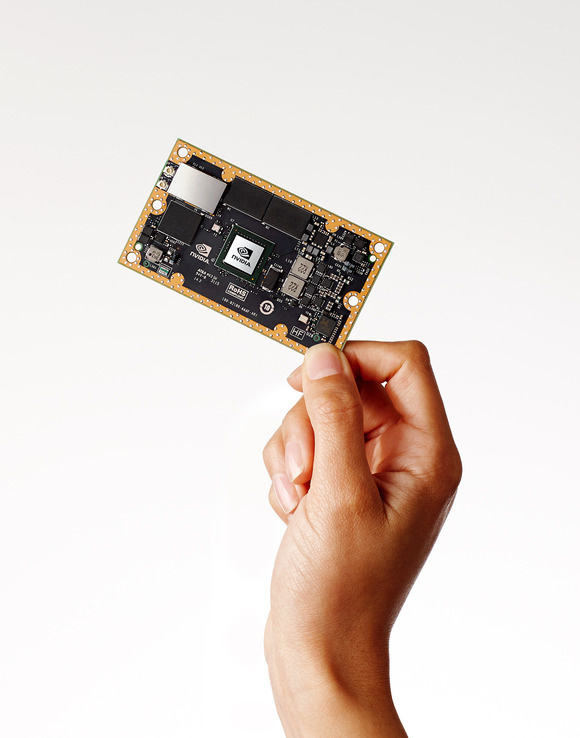
\includegraphics
        [height=5cm]
        {figures/jetson_scale.jpg}
    \caption{NVIDIA Jetson TX2 }\vspace{-4mm}
\end{figure}



\subsubsection*{Intel Realsense Depth Camera D435}

\begin{figure}[H]
    \centering
    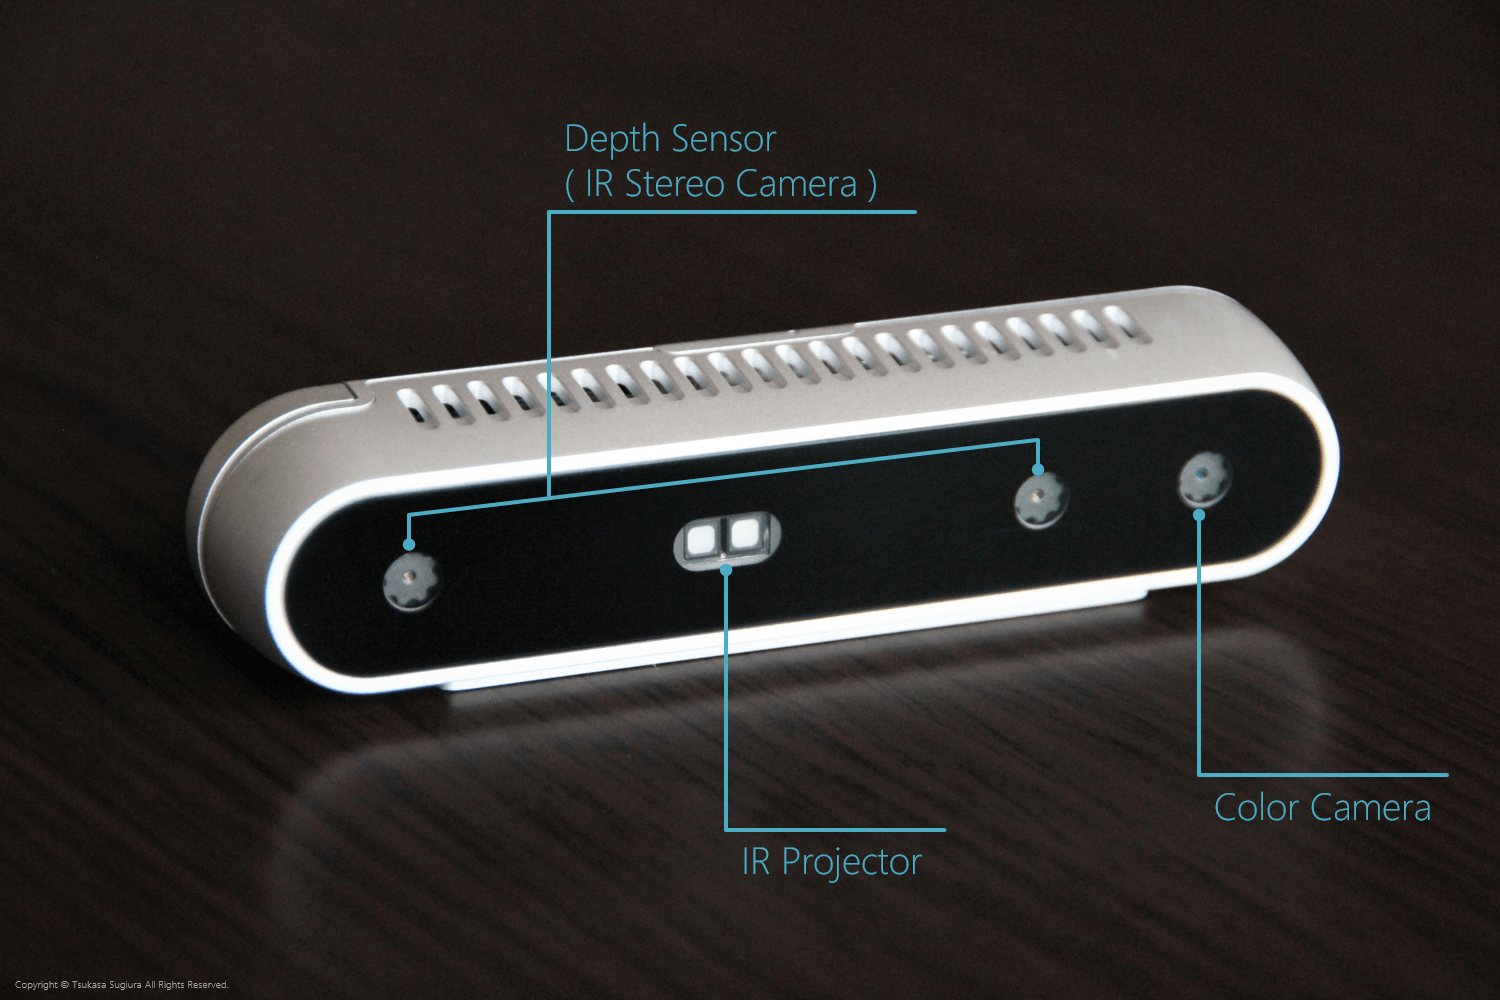
\includegraphics
        [width=12cm]
        {figures/realsense.png}
    \caption{Intel Realsense D435}\vspace{-4mm}
\end{figure}

\subsubsection*{Roboclaw Motor Controller}

\begin{figure}
    \centering
    \begin{minipage}{.5\textwidth}
        \centering
        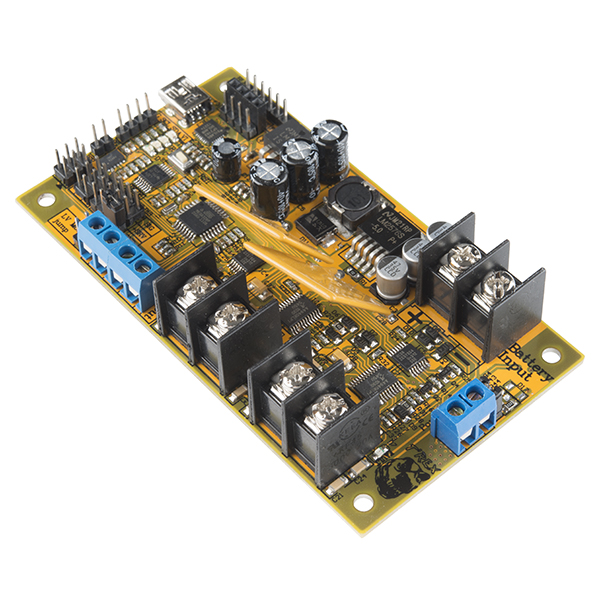
\includegraphics[width=\linewidth]{figures/trex.jpg}
        \captionof{figure}{TREX Motor Controller}
        \label{fig:test1}
    \end{minipage}%
    \begin{minipage}{.5\textwidth}
        \centering
        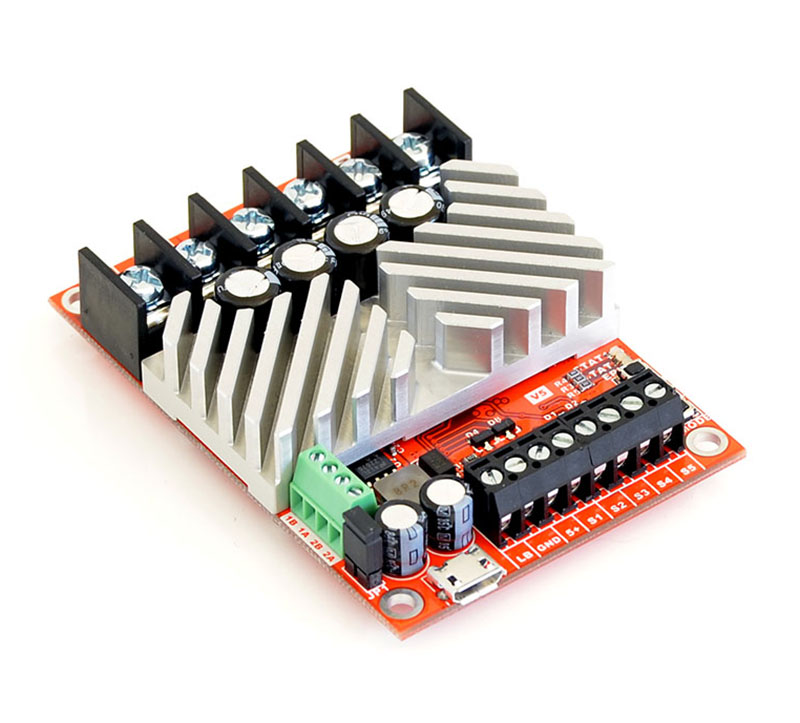
\includegraphics[width=\linewidth]{figures/roboclaw.jpg}
        \captionof{figure}{Roboclaw Motor Controller}
        \label{fig:test1}
    \end{minipage}
\end{figure}



\subsubsection*{Problems Faced and Solutions}





\newpage
\subsection{Designing and Implementing an Efficient End-toEnd Pipeline for Machine Learning in Robotics}

\begin{figure}[H]
    \centering
    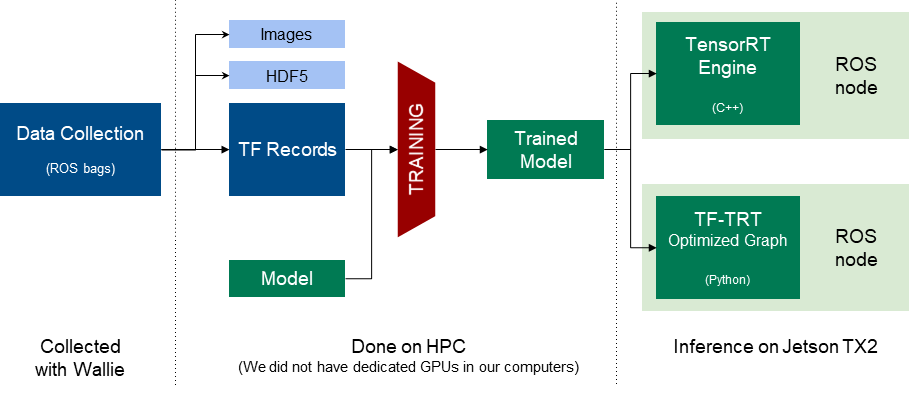
\includegraphics
        [width=16cm]
        {figures/full_pipeline.PNG}
    \caption{End-to-End Pipeline \label{Fig:pipeline}}\vspace{-4mm}
\end{figure}

\subsubsection{Training on Supercomputers}

\subsubsection{TF Records}

\begin{figure}[H]
    \centering
    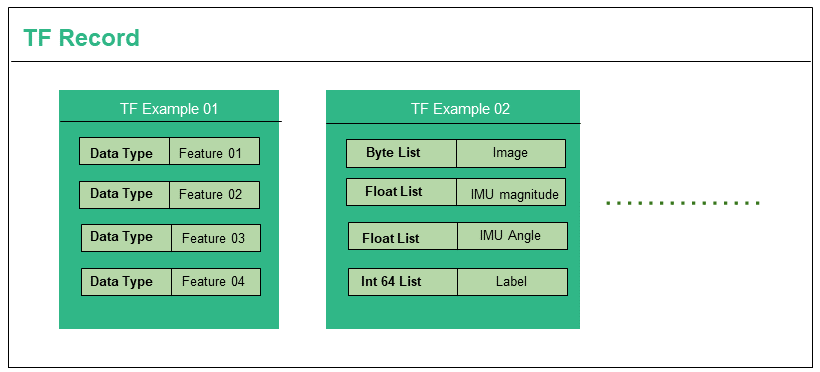
\includegraphics
        [width=9cm]
        {figures/tfrecord_structure.PNG}
    \caption{Structure of a TF Record}\vspace{-4mm}
\end{figure}

\subsubsection{TensorRT: Deployment on a low power device}

\begin{figure}[H]
    \centering
    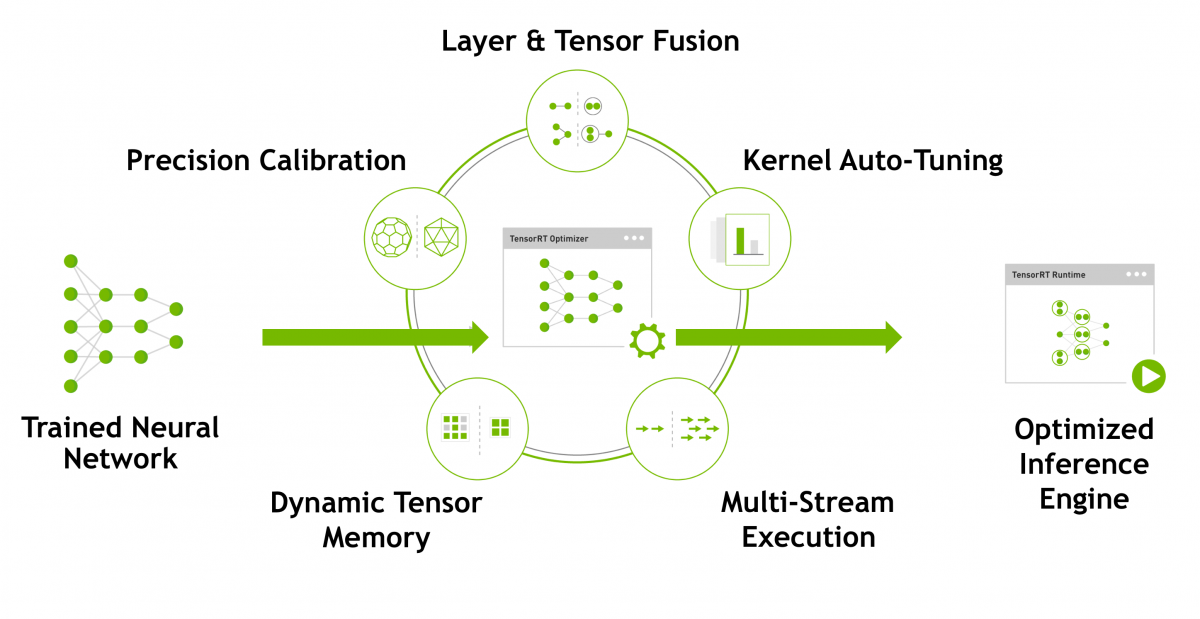
\includegraphics
        [width=13cm]
        {figures/trt.png}
    \caption{TensorRT in a nutshell}\vspace{-4mm}
\end{figure}

\begin{figure}[H]
    \centering
    
\includegraphics
        [width=13cm]
        {figures/deploy_pipeline_cpp.PNG}
    \caption{Deployment Pipeline: C++}\vspace{-4mm}
\end{figure}

\begin{figure}[H]
    \centering
    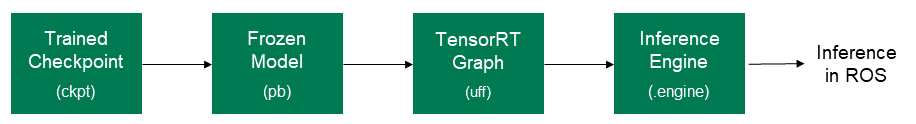
\includegraphics
        [width=13cm]
        {figures/deploy_pipeline_python.PNG}
    \caption{Deployment Pipeline: Python}\vspace{-4mm}
\end{figure}

\subsubsection{Problems Faced and Solutions}



\newpage
\subsection{Hillnet: An Experimental Attempt at Utilizing ML for Hill Climbing}

\subsubsection{Preprocessing IMU and Velocity Data}

\subsubsection{Classification Approach}

\subsubsection{Regression Approach}

\subsubsection{Merging Scaler and Image Inputs}

\subsubsection{Problems Faced and Solutions}



\newpage
\subsection{Life at CSIRO}
    

\subsubsection{Reading Groups and DATA61 Meetings}

\subsubsection{DATA61 Live Event}

\begin{figure}[H]
    \centering
    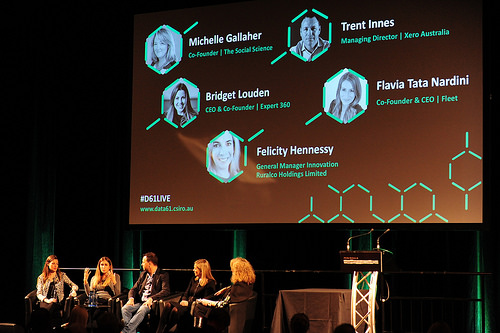
\includegraphics
        [height=5cm]
        {figures/data61_live_1.jpg}
    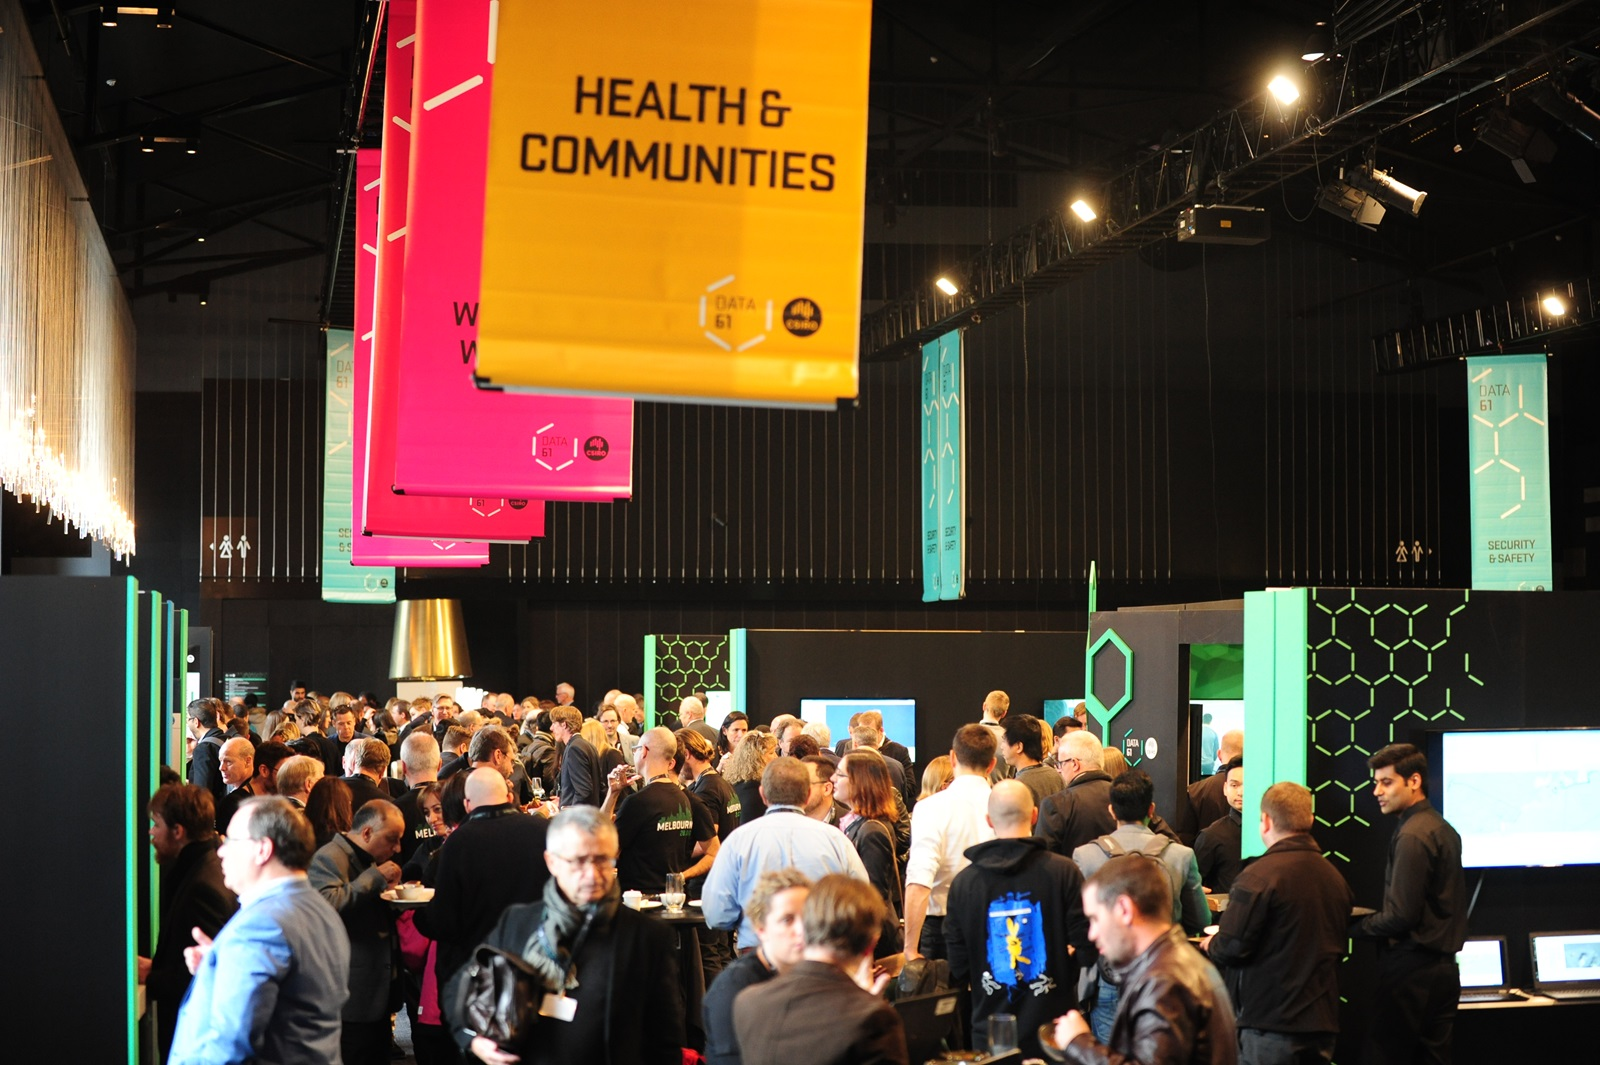
\includegraphics
        [height=5cm]
        {figures/data61_live_2.jpg}
    \caption{DATA61 LIVE Event}\vspace{-4mm}
\end{figure}


\newpage
\subsection{Presenting the Pipeline at Reading Group to the Scientists}



\newpage
\section{Conclusion}
%!TEX root = ./intern_report.tex

\paragraph{}
I worked as a research intern at DATA61 for 24 weeks. During this time, I worked three intertwined projects under the supervision of Nicolas Hudson and Dr. Navinda Kottege. 

\paragraph{}
The first project was developing indoor-Trailnet: a classification based approach to the autonomous navigation problem. For this, first I built a robot with Uvindu Perera for data collection and testing. We designed the power distribution system of the robot and assembled a high level and low level controllers. We calculated the torque requirements for the motors, current, voltage and power limitations for the power supply components and motor controllers during this process. We learnt a lot through debugging the errors we came across and extensively troubleshooting whenever a component or circuit board is damaged to provide a report on the event. I also debugged the driver software for the motor controller and modified parts of it to fix certain issues since it was not being maintained anymore.

\begin{figure}[H]
    \centering
    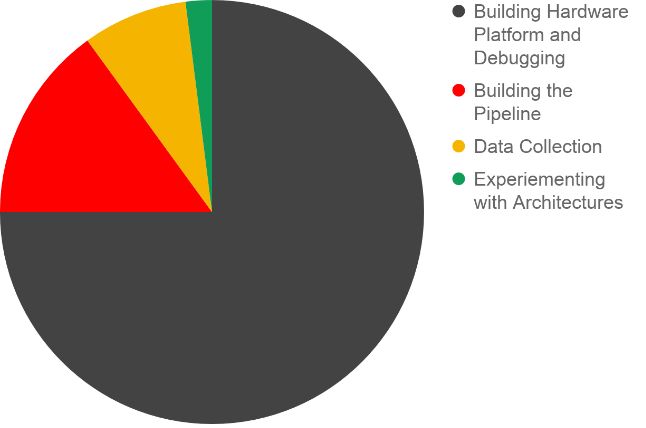
\includegraphics
        [width=9cm]
        {figures/time.PNG}
    \caption{Overview of our Time Spent}\vspace{-4mm}
\end{figure}

\paragraph{}
I learnt tensorflow and tensorflow-keras for this project and built a 20 layer residual network from scratch and trained it on the supercomputer cluster. Then I learnt tensorRT and deployed the trained network on Jetson TX2: a powerful embedded device that acted as the high level controller for the robot. I also learnt ROS (Robot Operating System) extensively, and created multiple ROS nodes and packages for testing, collecting data from sensors and for controlling the robot. 

\paragraph{}
For the next project of building an end to end pipeline for machine learning in robotics, I experimented and figured out the best practices when training models using large datasets on the supercomputer. I documented these experiments and the results, and proposed an efficient method to set up a writing and reading pipeline. I presented ~\cite{presentation} my pipeline in the Robotics Reading Group meeting. Many scientists were interested and some followed up via email asking questions and requesting to build tools for visualizing datasets.

\paragraph{}
The final project was experimental, where I explored different configurations of neural network architectures to build a robot that can climb hills while avoiding obstacles. Through literature survey and in-depth discussions with my supervisor, I learnt a lot about the structure of Deep Convolutional Neural Networks and possible methods of combining scaler data with the images to train a network. I tried several approaches here: solving the problem as a classification and a regression and using different ways to combine the inputs into the network. However, I was unable to get good results within the time we had there, due to the problems in data collection and the lack of time as we had to spend most of the time building and debugging the robot platform.

\paragraph{}
Also, I learnt about cross modal learning transfer and neural network distillation process through literature survey as a part of the project that was initially given, before we were changed into a different project a week later. Before and during the internship program, I expressed my interest in working in a project where I can develop algorithms and tackle abstract problems that could lead to new research and a publication. Unfortunately such a project was not available for interns at the time and my supervisors were satisfied with the work I was doing with hardware and deployment of machine learning. However, I learnt a lot through these projects and it had been a great experience. I also got familiarized with the software tools widely used in academia, high end sensors and controllers, and I daily worked with the Bracewell cluster, which is one of the world's largest supercomputer clusters. 

\paragraph{}
In addition to that, I learnt the etiquettes and responsibilities of working as an employee in a company. Helping others and asking for help, attending meetings and following up via official emails, documenting all the tasks and weekly progress in the wiki pages of CSIRO helped me learn a lot about these responsibilities. The work culture in DATA61 is exceptionally inclusive, where we got to work with people of multiple nationalities and share our culture. The students are allowed to work on their own pace and I was allowed to work overnight on multiple days and work on weekends as well. I also got to attend events such as DATA61 LIVE, where I could attend to many talks and discussion forums and observe the development of cutting edge technology of Australia through the exhibits.

\paragraph{}
From my experience, I would suggest DATA61 to assess the skills of the interns and assign them to projects relevant to those skills, to utilize their full potential for a project. Also, it would help if they can give an overview of the project at the beginning of the internship and set incremental goals to be completed at given deadlines. I found it disorienting when the project given to me before the internship was changed as I reached there and changed again a week later to settle on an experimental project of my supervisor that subsequently evolved into the three above projects (that I explained in Chapter 2) through the period of six months. 

\paragraph{}
I would also like to suggest NAITA to computerize the supervision process, where interns can submit the intern diary and monthly reports online. This would help because in organizations like CSIRO, the students are expected to maintain an online diary and the interns can save time by writing by hand the same thing they have typed into the online diary.

\paragraph{}
Therefore, I can conclude that my overall experience in DATA61 was great. I had the opportunity to learn a lot and make contacts. I am deeply thankful to the Industrial Training Division of our university and NAITA for this internship and I am thankful for DATA61 and my supervisors for providing me with such an exceptional opportunity and a training experience.








\end{document}